\documentclass{beamer}


\usepackage{tikz}
\usetikzlibrary{shapes,arrows,positioning}
\usetikzlibrary{snakes}
\usepackage{textpos}
\usepackage{calc}
\usepackage{graphicx,color,psfrag,epsfig}
\usepackage{setspace}
\beamertemplatenavigationsymbolsempty

\usepackage{textcomp}

\usepackage{mathtools}
\usepackage{sansmath}

\usefonttheme{professionalfonts}
\usefonttheme{serif}
\usepackage{fontspec}
\setmainfont{Arial}

% To make the navigation bullets appear
\usepackage{remreset}
\makeatletter
    \@removefromreset{subsection}{section}
\makeatother
\setcounter{subsection}{1}

\setbeamersize{text margin left=3mm, text margin right = 3mm} 

\usetheme{default}
\useoutertheme[subsection=false]{smoothbars}

\xdefinecolor{darkgreen}{rgb}{0,0.35,0.05}
\usecolortheme[named=white]{structure}

%Custom commands
%Absolute figure/text placement
\newcommand{\putat}[3]{\begin{picture}(0,0)(0,0)\put(#1,#2){#3}\end{picture}} 

\mode<presentation> 

\linespread{1.2}

\begin{document}


% Title Slide 
%	{\setbeamertemplate{background canvas}{\includegraphics[width=\paperwidth,height=\paperheight]{figures/arthurs_cataract.jpg}}


\setbeamercolor{background canvas}{bg=black}
\setbeamercolor{normal text}{fg=white,bg=}
\setbeamercolor{example text}{fg=white,bg=}
\usebeamercolor[fg]{normal text}

\begin{frame}[plain]
	\begin{center}
		{\LARGE{Traffic patterns on mountain passes}} \\
		\vspace{2em}
		\includegraphics[width=0.5\textwidth]{figures/mountains.png} \\
		\vspace{1em}
		{\Large{\color{white}{Laura Kehrl}}}
	\end{center}
\end{frame}

\begin{frame}[plain]
	\begin{columns}
		\begin{column}{0.45\textwidth}
			\Large{Over 20,000 cars and trucks travel over mountain passes in WA state each day.}  \\
			\vspace{2em}
			Can we use historical traffic data to predict the busiest hours on a given day? \\
		\end{column}
		\begin{column}{0.4\textwidth}
			\includegraphics[width=\textwidth]{figures/snoqualmie_summer_wsdot.jpg} \\
			\vspace{1em}
			\includegraphics[width=\textwidth]{figures/snoqualmie_winter_wsdot.jpg}
		\end{column}
	\end{columns}
	\begin{textblock}{6}(8.6,-6.5)
		{\tiny{\color{black}{\copyright WSDOT}}}
	\end{textblock}
	\begin{textblock}{6}(8.6,-0.4)
		{\tiny{\color{black}{\copyright WSDOT}}}
	\end{textblock}
\end{frame}

\begin{frame}[plain]
	\vspace{0.3em}
	\begin{columns}
		\begin{column}{0.95\textwidth}
			{\Large{Hourly traffic data from WSDOT}}
		\end{column}
	\end{columns}
	\vspace{0.2em}
	\includegraphics[width=\textwidth]{figures/WA_state_map.pdf}
	\vspace{-0.5em}
		\begin{columns}
		\begin{column}{0.4\textwidth}
			\large{\begin{itemize}
				\item Vehicle type and count since 2007 \\ {\normalsize{(1,000,000+ rows)}}
			\end{itemize}}
		\end{column}
		\begin{column}{0.4\textwidth}
			\large{\begin{itemize}
				\item Vehicle speed \\ since 2016 \\ {\normalsize{(750,000+ rows)}}
			\end{itemize}}
		\end{column}
	\end{columns}
\end{frame}

\begin{frame}[plain]
	\vspace{0.5em} 
	\Large{An example: Sundays on Snoqualmie Pass}
	\vspace{0.9em}
	\begin{columns}
	\begin{column}{0.02\textwidth}
	\end{column}
	\begin{column}{0.36\textwidth}
		\large{Why does the distribution of busiest hours vary over the year?} \\
		\vspace{7em}
	\end{column}
	\begin{column}{0.3\textwidth}
		\large{\centerline{Eastbound}} \\
		\vspace{0.2em}
		\includegraphics[width=1\textwidth]{figures/S901_Eastbound_January_Sunday.pdf} \\
		\includegraphics[width=1\textwidth]{figures/S901_Eastbound_August_Sunday.pdf}
	\end{column}
	\begin{column}{0.3\textwidth}
		\large{\centerline{Westbound}} \\
		\vspace{0.2em}
		\includegraphics[width=1\textwidth]{figures/S901_Westbound_January_Sunday.pdf} \\
		\includegraphics[width=1\textwidth]{figures/S901_Westbound_August_Sunday.pdf} 
	\end{column}
	\begin{column}{0.02\textwidth}
	\end{column}
	\end{columns}
\end{frame}

\begin{frame}[plain]
	\begin{columns}
	\begin{column}{0.95\textwidth}
	\vspace{0.5em} \\
	\Large{Ski areas on mountain passes \\ affect traffic patterns}  \\
	\vspace{1.5em}
	\includegraphics[width=\textwidth]{figures/Snoqualmie_vehicles_on_pass.pdf}
	\end{column}
	\end{columns}
	\begin{textblock}{6}(10.5,-15)
		\includegraphics[width=1.5in]{figures/skiing.png} \\
	\end{textblock}
	\vspace{1em}
	\footnotesize{\centerline{Code for all plots available at https://github.com/kehrl/mountain-traffic}}
\end{frame}

\begin{frame}[plain]
	\Large{Can we predict the busiest hours to travel on a given day?} \\
	\vspace{2.5em}
	\Large{Feature selection}
	\large{
	\begin{itemize}
		\item Travel Direction
		\item Daylight hours
		\item Ski resort open
		\item Holiday 
		\item Week day 
	\end{itemize}
	}
	\vspace{3em}
	\begin{textblock}{12}(9,-9.5)
		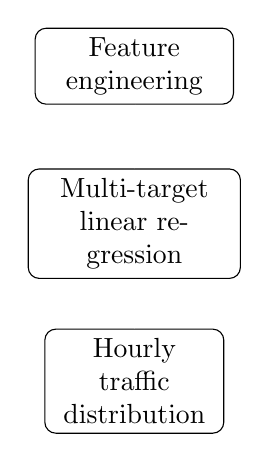
\begin{tikzpicture}[node distance = 2.0cm, auto]
			\node  [rectangle, draw,
    minimum width, rounded corners,fill=white,text=black,text width=6.5em,align=center] (feature) {\normalsize{Feature engineering}};
    			\node [rectangle, draw,minimum width, rounded corners, below of=feature,,fill=white,text=black,text width=7em,align=center] (model) {\normalsize{Multi-target linear regression}};
			\path [draw, -latex',line width=1.5pt,white] (feature) -- (model);
			\node [rectangle, draw, rounded corners, below of=model,fill=white,text=black,text width=5.8em,align=center] (input) {\normalsize{Hourly traffic distribution}};
			\path [draw, -latex',line width=1.5pt,white] (model) -- (input);
		\end{tikzpicture}
	\end{textblock}
\end{frame}

\begin{frame}[plain]
	\Large{Users want to avoid busy hours \emph{and} road closures.} \\
	\vspace{0.5em}
	\begin{columns}
	\begin{column}{1\textwidth}
		\includegraphics[width=1\textwidth]{figures/twitter_example.png}
	\end{column}
	\end{columns}
	\vspace{0.5em}
	Can we predict when a mountain pass will be closed based on current weather observations?
\end{frame}

\end{document}

